\subsubsection{Modelo de comportamiento menú principal}

\textbf{Diagrama de secuencia}
\begin{figure}[H]
  \label{dia_menu_principal}
  \begin{center}
    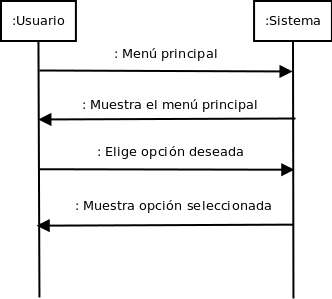
\includegraphics[scale=0.5]{imagenes/dia_menu_principal.png}
  \end{center}
  \caption{Análisis: Diagrama de secuencia Menú principal}
\end{figure}

\textbf{Contrato operaciones}

\begin{description}
    \item[Operación] Menú principal
    \item[Actores] Usuario, Sistema
    \item[Responsabilidades] Selecciona la opción principal del juego.
    \item[Precondiciones] Ninguna
    \item[Postcondiciones] Ninguna
\end{description}

\subsubsection{Modelo de comportamiento elegir personaje}

\textbf{Diagrama de secuencia}
\begin{figure}[H]
  \label{dia_elegir_jugador}
  \begin{center}
    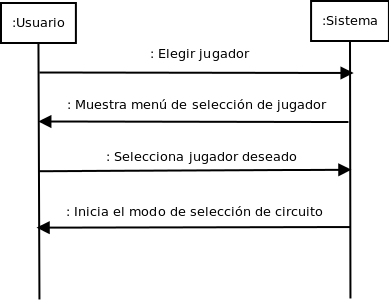
\includegraphics[scale=0.5]{imagenes/dia_elegir_jugador.png}
  \end{center}
  \caption{Análisis: Diagrama de secuencia Elegir jugador}
\end{figure}

\textbf{Contrato operaciones}

\begin{description}
    \item[Operación] Elegir personaje
    \item[Actores]  Usuario, sistema
    \item[Responsabilidades] Selecciona el personaje a controlar en el juego.
    \item[Precondiciones] Ha elegido previamente uno de los modos de juego en el menú principal.
    \item[Postcondiciones] Selecciona al personaje.
\end{description}

\subsubsection{Modelo de comportamiento elegir circuito}

\textbf{Diagrama de secuencia}
\begin{figure}[H]
  \label{dia_elegir_circuito}
  \begin{center}
    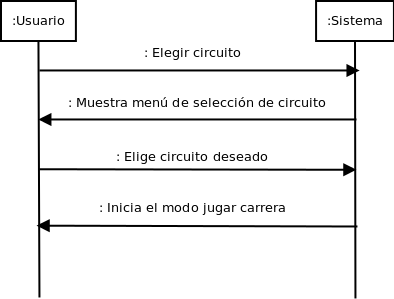
\includegraphics[scale=0.5]{imagenes/dia_elegir_circuito.png}
  \end{center}
  \caption{Análisis: Diagrama de secuencia Elegir circuito }
\end{figure}

\textbf{Contrato operaciones}

\begin{description}
    \item[Operación] Elegir circuito
    \item[Actores] Usuario, sistema
    \item[Responsabilidades] Selecciona el circuito donde competirá el jugador.
    \item[Precondiciones] Ha elegido previamente el personaje que competirá y el modo de juego carrera rápida o contrarreloj
    \item[Postcondiciones] Selecciona el circuito.
\end{description}

\subsubsection{Modelo de comportamiento elegir campeonato}

\textbf{Diagrama de secuencia}
\begin{figure}[H]
  \label{dia_elegir_campeonato}
  \begin{center}
    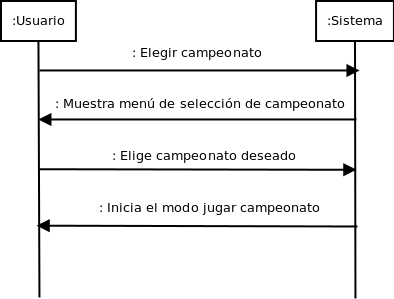
\includegraphics[scale=0.5]{imagenes/dia_elegir_campeonato.png}
  \end{center}
  \caption{Análisis: Diagrama de secuencia Elegir campeonato}
\end{figure}

\textbf{Contrato operaciones}

\begin{description}
    \item[Operación] Elige campeonato
    \item[Actores] Usuario, sistema
    \item[Responsabilidades] Seleccionar el campeonato en el que competirá el jugador.
    \item[Precondiciones] Ha elegido previamente el personaje que competirá y el modo de juego campeonato.
    \item[Postcondiciones] Selecciona el campeonato.
\end{description}

\subsubsection{Modelo de comportamiento jugar carrera}

\textbf{Diagrama de secuencia}
\begin{figure}[H]
  \label{dia_jugar}
  \begin{center}
    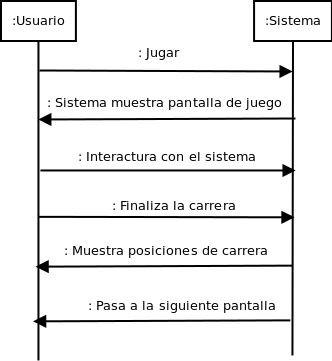
\includegraphics[scale=0.5]{imagenes/dia_jugar.png}
  \end{center}
  \caption{Análisis: Diagrama de secuencia Jugar carrera}
\end{figure}

\textbf{Contrato operaciones}

\begin{description}
    \item[Operación] Jugar
    \item[Actores] Usuario, sistema
    \item[Responsabilidades] Muestra la pantalla de juego desde la que el usuario puede jugar la partida.
    \item[Precondiciones] Previamente se han elegido jugador y circuito.
    \item[Postcondiciones] Un jugador gana la carrera.
\end{description}

\subsubsection{Modelo de comportamiento jugar campeonato}

\textbf{Diagrama de secuencia}
\begin{figure}[H]
  \label{dia_jugar_campeonato}
  \begin{center}
    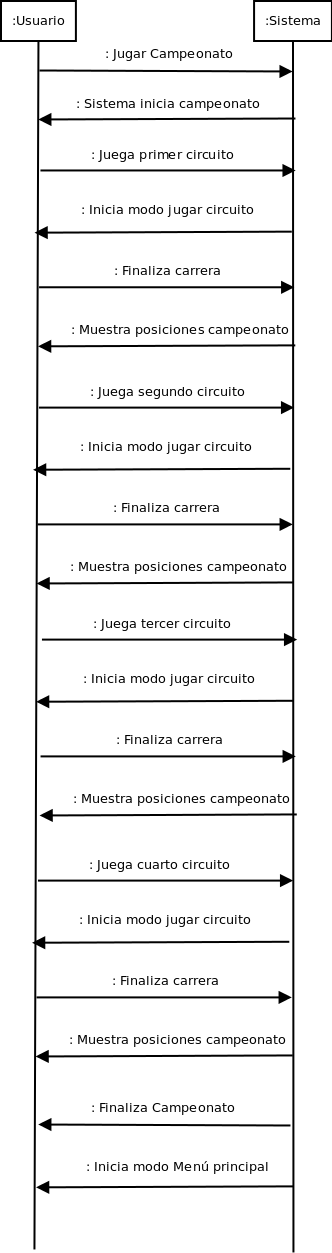
\includegraphics[scale=0.5]{imagenes/dia_jugar_campeonato.png}
  \end{center}
  \caption{Análisis: Diagrama de sencuancia Jugar campeonato}
\end{figure}

\textbf{Contrato operaciones}

\begin{description}
    \item[Operación] Jugar Campeonato
    \item[Actores] Usuario, sistema
    \item[Responsabilidades] Desarrolla todas la carreras del campeonato
    \item[Precondiciones] Se eligió el modo campeonato en el menú principal.
    \item[Postcondiciones] Un jugador gana el campeonato.
\end{description}

\subsubsection{Modelo de comportamiento opciones}

\textbf{Diagrama de secuencia}
\begin{figure}[H]
  \label{dia_opciones}
  \begin{center}
    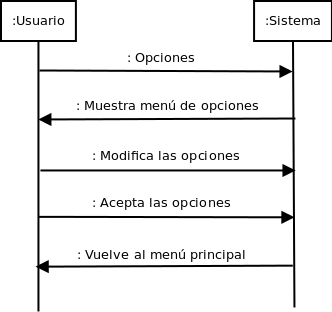
\includegraphics[scale=0.5]{imagenes/dia_opciones.png}
  \end{center}
  \caption{Análisis: Diagrama de secuencia opciones}
\end{figure}

\textbf{Contrato operaciones}

\begin{description}
    \item[Operación] Opciones
    \item[Actores] Usuairo, sistema
    \item[Responsabilidades] Se muestran las distintas opciones que el usuario puede modificar, como son el audio, pantalla y
    controles.
    \item[Precondiciones] Ninguna
    \item[Postcondiciones] Se modifican las opciones del juego.
\end{description}

\subsubsection{Modelo de comportamiento salir}

\textbf{Diagrama de secuencia}
\begin{figure}[H]
  \label{di_salir}
  \begin{center}
    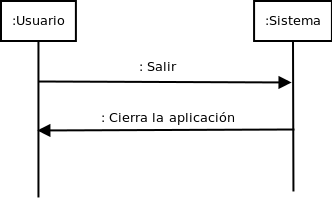
\includegraphics[scale=0.5]{imagenes/dia_salir.png}
  \end{center}
  \caption{Análisis: Diagrama de secuencia Salir}
\end{figure}

\textbf{Contrato operaciones}

\begin{description}
    \item[Operación] Salir
    \item[Actores] Usuario, Sistema
    \item[Responsabilidades] Permite al usuario salir del sistema
    \item[Precondiciones] Ninguna
    \item[Postcondiciones] Se sale de la aplicación
\end{description}
